\chapter{Analysing GDPR Compliance Requirements}
\label{chapter:information}

The analysis of state of the art in \autoref{chapter:sota} provided identification of opportunities for addressing the gaps within it.
These opportunities relate to the research objectives $RO3$ regarding construction of ontologies, $RO4$ for querying, and $RO5$ for information validation.
In order to achieve these, it is imperative to have an understanding of the GDPR and its compliance requirements as required by research objective $RO1$.
The requirement gathering process is shaped by the scope of the research question - which for this thesis is regarding the representation of activities associated with processing of personal data and consent.
The identified requirements then need to be expressed in a form which will facilitate the representation of information as ontologies and its querying and validation in the compliance process. This is required to fulfil research objective $RO2$.

The approaches within the state of the art presents their work in relation to the requirements of GDPR compliance primarily associated with either the data subject or data controller.
In reality, the requirements of compliance are also influenced by the other stakeholders - such as processors and authorities which play an unspecified role in the context of information associated with compliance.
Such roles consist of interactions between stakeholders which involve communication of information such as the instructions provided by a data controller to a processor.
Therefore along with the requirements of compliance, it is also important to understand the interactions between stakeholders, the information involved in such interactions, and the requirements of information in terms of its interoperability between them.
Such analyses and requirements gathering related to the GDPR benefit the larger community and domain by providing the background for standardisation activities in understanding the role of information and its interoperability between stakeholders, such as those for DPVCG \autoref{sec:intro:dpvcg}.

This chapter therefore first presents an analysis of GDPR in terms of stakeholders and interoperability of information between them along with an analysis of suitability of existing standards to represent it in \autoref{sec:info:model}.
Following this, \autoref{sec:info:compliance-questions} frames `compliance questions' that provide information requirements necessary to evaluate compliance, with the methodology presented in \autoref{sec:info:compliance-questions-methodology}, and \autoref{sec:info:constraints} presenting assumptions and constraints that can be used to validate the information for correctness and completeness.
The use of compliance questions as competency questions in the development and evaluation of ontologies is presented in \autoref{chapter:vocabularies}, and the use of constraints for validations is presented in \autoref{chapter:testing}.

\section{Interoperability Model of Information based on GDPR}\label{sec:info:model}

This section presents an analyses of the GDPR in terms of interactions between stakeholders and the information involved in such interactions. It then presents a model of interoperability for information associated with stakeholders. The model enables understanding the role of stakeholders in the compliance process in terms of information requirements and provides a framework to establish the relationship between the interactions and information required for compliance. 
The model also provides motivation to incorporate interoperability as a core requirement within representations of information towards GDPR compliance.
The work described in this section was published within the interoperability and standardisation community as a conference paper
\cite{pandit_gdpr_2018} which was later expanded upon in a journal article \cite{pandit_exploration_2018} and a book chapter \cite{pandit_standardisation_2020}.

The categorisation of stakeholders (or entities) in terms of GDPR compliance are visualised in Figure \ref{fig:info:interoperability-model} and consist of Data Subject (DS), Data Controller (DC), Data Processor (DP) and Supervisory Authority\footnote{Supervisory Authority are also referred to as Data Protection Commission or Regulatory Body} (SA). 
The figure also mentions Data Management (DM) as a type of virtual entity provided by a third party in the form of a product, tool, or service whose function is to provide an interface to the controller or processor for assisting and automating their operations. 
Although the GDPR does not mention or allude to the existence or functionality of DM, it is included based on the information interoperability requirements it represents as required by the operating controller or processor.
\begin{figure}[htbp]
    \centering
    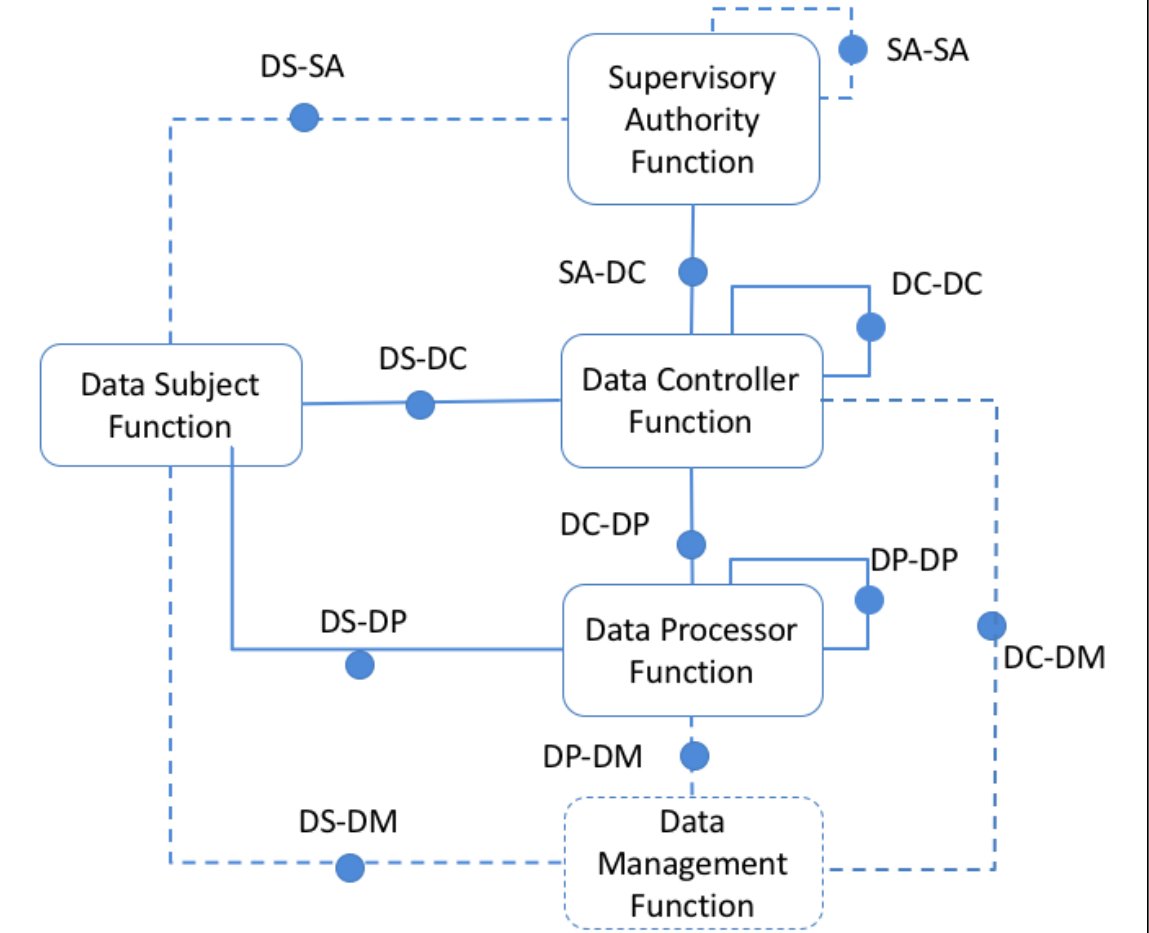
\includegraphics[width=0.75\linewidth]{img/interoperability-model.png}
    \caption{Model of information interoperability between entities based on requirements of GDPR \cite{pandit_exploration_2018}}
    \label{fig:info:interoperability-model}
\end{figure}

With this, there are 11 possible points of interactions between entities as indicated by the blue dots in the figure with the label specifying the two entities involved in an interaction.
The interactions are considered directionless, and use the abbreviations defined above. For example, DC-DP represents an interaction between a data controller and a data processor.
The solid line corresponds to interactions defined by the GDPR between stakeholders, while the dotted lines represent interactions derived from information interoperability requirements.
Where a cyclic interaction is specified, such as DC-DC occur between the same type of stakeholder, they represent interactions between different organisations of the same type, which in this case means two different data controllers.

The points of interactions consist of information exchange between entities, are are guided by the requirements of compliance. For example, the interaction between data subject and data controller consists of the data subject providing personal data to the controller, while the controller is required to provide a copy of provided personal data for fulfilment of rights granted by the GDPR.

Analyses of information flows between entities enables categorisation of requirements across the categories of provenance records, consent information, data processing agreements, compliance information, and use of seals/certifications \cite{pandit_exploration_2018}.

\subsubsection*{Provenance records}
Provenance in this case refers to information about entities and activities involved in the compliance process, where a record is required to be kept and exchanged for compliance purposes. For example, GDPR requires controllers and processors to maintain provenance records of processing activities carried out under their responsibility in order to maintain and demonstrate compliance to supervisory authorities. Provenance records are also required to be maintained to enable provision of rights to the data subject, and for information sharing between controllers and third parties.

The information stored within provenance records is related to demonstrating compliant processing of personal data and fulfilment of obligations towards demonstration of compliance. They are modelled within the state of the art (see \autoref{chapter:sota}) variously as logs, life-cycles, workflows, activities, and process flows. The term provenance in this case refers to both ex-ante and ex-post phases and is indicative of provenance of information to specify its existence. Therefore provenance in ex-ante phase would mean the record of a model or plan used to indicate future processing of personal data.

Since provenance information as described above encompasses information about artefacts and processes related to compliance, sharing this information in an interoperable format with other entities benefits both in their obligations regarding compliance. For example, controllers  and supervisory authorities sharing interoperable compliance documentation can use the same set of tools and approaches for interacting with the information. Also, by recording the processes associated with compliance as provenance records, the same interoperable methods can be used to maintain, document, and demonstrate the compliance. This is especially useful where information is to be shared between joint controllers and processors that need to exchange plans of processing for agreement as well as logs for successful implementations.

\subsubsection*{Data Processing Agreements}
A controller and processor, or controller and another controller, or processor and another processor - are required to have specific data processing agreements in place that specify the processing activities to be carried out. 
In such agreements, the first entity specifies the processing to be carried out, and the second entity is obliged to carry out processing within the scope of received instructions. The GDPR differentiates between a controller and processor based on the freedom to determine the purpose of processing, where a controller can determine such purposes independently while a processor must follow instructions received from a controller.

The provision of instructions from one entity to another need to be recorded by both parties for compliance purposes, and to demonstrate the exact processing operations they are authorised to carry out. GDPR also requires inclusion of information in data processing agreements regarding certain measures such as security safeguards for the processing of personal data. The entity that processes data may also be required to confirm or communicate its fulfilment of instructions under the terms of the agreement, such as when there are obligations for immediate erasure of data following completion of processing operations. Another case is when data is being processed on the basis of consent, the withdrawal of revocation of consent requires such processing to be halted and in some cases the personal data to be erased. When a processor is utilised to process personal data, revocation of consent need to be communicated in order to ensure halting of processing and removal of personal data.

From this, it is evident that data sharing agreements contain information about processing activities, and can be expressed as process flows in both ex-ante and ex-post phases. Here, ex-ante phase refers to the agreement itself where both entities agree on the processing to be carried out, while ex-post information concerns with the completion of processing.

\subsubsection*{Consent information}
As per GDPR, consent is an assent or agreement by the data subject regarding the processing of their personal data for specified purposes by one or more entities. 
For compliance, a controller must record information regarding how consent was requested and the choices provided by the data subject in the form of given consent.
GDPR has several obligations and requirements when it comes to valid consent, with additional requirements depending on the sensitivity of personal data and processing. 
Artefacts associated with choices offered for consent therefore need to be preserved to demonstrate the validity of consent obtained using those choices.
Similarly, consent revocation or revisions also need to be similarly stored and linked to the original consent to demonstrate the change was valid as per the requirements of the GDPR.

The processes associated with offering consent choices, retrieving and recording given consent, enabling withdrawal of consent, and executing revocation in internal processes need to thus be documented for compliance by the relevant controller(s).
These are associated across both ex-ante and ex-post phases where consent choices, provision of right to withdrawal, and demonstrating utilisation of consent in processing are demonstrated as ex-ante measures while given consent and revoked consent are ex-post artefacts. 

If consent is considered as an instance of personal data, the same information model used to document processing of personal data can be re-purposed to represent activities associated with consent. In addition to this, the activities need to capture the various stages of consent and personal data by representing their life-cycles which involve processes and artefacts which use them or are dependant on them. The 

\subsubsection*{Compliance documentation}
Controllers and processors need to maintain ongoing compliance, including documentation of the compliance assessment process. Therefore, compliance as per the GDPR is a continuous process and requires presence of processes or activities that carry out periodic checks of compliance starting from the planning stage to the execution of activities.
When a new service or process is to introduced or an existing process is changed, their compliance is required to be determined and documented prior to their execution.
Such checks may be carried out as part of internal audits or periodic reviews, whose documentation should reflect the outcomes of compliance, and any remedial measures carried out.

The processes associated with compliance involve information about processing activities and can be represented using the same information model as processing activities by including additional information required for the compliance process. Periodic changes or checks can be persisted as provenance records that can act as documentation of compliance processes and the state of compliance at a particular time.

\subsubsection*{Use of certifications}
GDPR provides for seals and certifications to be used to denote a certain degree of compliance based on existence of measures and processes indicated by the seal of certification. The presence of such seals and certifications as well as their associated information needs to be exchanged between entities to demonstrate trust and guarantees, such as between processors and controllers, or controllers and data subjects. Seals and certifications indicate a common criteria which is known to entities and supervisory authorities in order to register its use. The exact role of seals and certifications in the compliance process is still under consideration by the authoritative bodies, and is expected to be clarified in the coming period.

\subsubsection*{Opportunities for commonality and interoperability}
The model and analyses of information flows between entities provides the motivation for establishing interoperability in the representation of information to be exchanged.
In particular, provenance records regarding activities associated with processing of personal data and consent are relevant in all interactions, and consequently are important to the documentation of compliance for all stakeholders. 

Representing provenance is not limited to representation of processing of personal data, but is also applicable to information about other categories - consent, data processing agreements, compliance, and certifications. Therefore, utilising the same or compatible representation in representing provenance for all categories has advantages of utilising a cohesive management of all associated information towards compliance.

The representation of activities in the ex-ante and ex-post phases associated with processing of personal data is well established based on the analysis of state of the art (see \autoref{sota:analysis:process-flows}). 
Approaches have utilised existing standards such as PROV and BPMN to represent information in an interoperable form. 
While this provides the potential to reuse the same representation towards other information categories described above, the approaches within the SotA do not exploit this opportunity.

As the scope of the thesis focuses on representation of activities associated with processing of personal data and consent, the requirements gathered from this analysis relate primarily to the information associated with provenance of activities and information about consent.
Within this scope, the effort of ensuring potential reuse towards other categories through future extensions is provided by developing an interoperable ontology by using standards that can be utilised to also represent data processing agreements and compliance agreements in the future.
This involves using standards such as RDF and OWL2 to represent the ontology, and the reuse of existing standardised vocabularies such as PROV-O and ELI.
In addition, the research also provides transparency by using terminology of GDPR in the developed ontologies, indicating the requirements used to shape the design of ontology, and indicating the source of concepts within GDPR.

With this motivation, the next parts of this chapter provide the requirements gathered for representing information regarding processing of personal data and consent, while also including other relevant information - such as data breaches and provision of rights - to indicate the potential applicability and reuse of developed ontologies in representing additional information for GDPR compliance.

\section{Compliance Questions}\label{sec:info:compliance-questions}
This section presents `compliance questions' whose answers provide information necessary for evaluating GDPR compliance. The questions are essential to the development of information representations within compliance management systems by providing requirements for the structuring of information and its validation. Within this thesis, they are used to guide the development of ontologies as competency questions (see \autoref{chapter:vocabularies}) and validation of information (see \autoref{chapter:testing}). The questions presented here are by no means exhaustive but represent gathered requirements from authoritative sources. As supervisory authorities and courts continue to clarify and interpret the compliance requirements of GDPR, these questions are expected to change and expand in the future.

\subsection{Methodology}\label{sec:info:compliance-questions-methodology}
The questions were collected from authoritative sources such as data protection commissions, legal experts and agencies - that have published guidelines and resources to assist organisations with the process of establishing and maintaining GDPR compliance.
Some resources - such  as checklists or criteria to self-assess measure of GDPR compliance within an organisation - already provide questions which were adopted for use. In other cases, questions were derived from the reading and understanding of compliance requirements. 

For the questions presented in this thesis, the following sources were used or referenced in addition to the text of GDPR:
\begin{itemize}
    \item Guidelines, clarifications, and discussions on the interpretation of GDPR published by European Data Protection Board\footnote{\url{https://edpb.europa.eu/}} (EDPB)
    \item Guidelines, clarifications, and discussions on the interpretation of GDPR published by Article 29 Working Party\footnote{\url{https://ec.europa.eu/newsroom/article29/news.cfm?item_type=1360}} and endorsed by EDPB
    \item Resources published Data Protection Commission\footnote{\url{https://dataprotection.ie/}} (Ireland) - with particular focus on document `GDPR guidance for SMEs'\footnote{\url{https://dataprotection.ie/en/guidance-landing/guidance-smes}}
    \item Resources published by Information Commissioners Office\footnote{\url{https://dataprotection.ie/}} (United Kingdom), with particular use of `Data protection self assessment for organisations'\footnote{\url{https://ico.org.uk/for-organisations/data-protection-self-assessment/}}
    \item Resources published by federated data protection offices in Germany, in particular the audit checklist published by Lower Saxony Data Protection Authority\footnote{\url{https://lfd.niedersachsen.de/download/146715/}} which was self-translated from German to English\footnote{\url{https://doi.org/10.5281/zenodo.3380469}}
    \item Resources regarding GDPR compliance published by professional institutions within legal compliance domain, specifically - Nymity\footnote{\url{https://info.nymity.com/gdpr-compliance-toolkit}} and IAPP\footnote{\url{https://iapp.org/resources/article/gdpr-genius/}}
    \item Executive and Court decisions regarding GDPR compliance, tracked using the online community service \url{https://www.enforcementtracker.com/} which also provides the article of GDPR relevant to the decision
\end{itemize}

The collected questions were rephrased and divided into smaller more granular questions towards establishment of information requirements and constraints. 
Each question was assigned an ID to enable tracking its use.
Where possible, each question was associated with specific clauses of the GDPR by denoting the article or recital relevant to it. Each question was analysed in terms of information requirements to identify assumptions that clarify interpretation of the question, and constraints that express a condition that can be tested and used to validate the information. For each identified constraint, a failing test case was identified that did not satisfy the condition and could be used to test its validation.
% \todo{upload all documents to Zenodo and put link here}
% A spreadsheet was used to collect and organise the questions, assumptions, and constraints - and is available as an open resource\footnote{\url{TODO: upload spreadsheet to Zenodo and post link here}}.

The list of questions is presented in \autoref{sec:info:compliance-questions-list} with the assumptions and constraints presented in \autoref{sec:info:constraints}. Along with compliance questions regarding activities associated with processing of personal data and consent, the list also contains questions about additional activities associated with right to be informed and reporting of data breach by controllers. These are later used in the development of ontologies that demonstrate the application of a common approach to represent activities related to processing of personal data, consent, data breach, and provision of rights for GDPR compliance. 

\subsection{List of Questions}\label{sec:info:compliance-questions-list}

\subsubsection{Use-cases}
To identify the application of compliance questions in various scenarios within the real world, 15 categories of use-cases were identified to determine the necessary information required to identify their ontological representations.
The use-cases are based on identifying information affecting compliance requirements and identifying variances which affect the representations of that information.
These were useful to guide the development of the ontology by serving as test scenarios where an ontology could be applied and evaluated for representing information.
These use-cases are not intended to be comprehensive or normative.

A summary of these use-cases is as follow:
\begin{enumerate}
% \tightlist
\item
  Obtaining / Declaring Consent (its state)

  \begin{enumerate}
%   \tightlist
  \item
    The consent is given
  \item
    Consent was given, but is now invalidated (by the controller)
  \item
    Consent was given, but was withdrawn (by the Data Subject)
  \item
    Consent was requested (by the controller)
  \item
    Consent was requested, but was refused (by the Data Subject)
  \item
    Consent state is unknown (e.g. when importing data about consent)
  \end{enumerate}
\item
  Entity the consent is about

  \begin{enumerate}
%   \tightlist
  \item
    The consent is about a Data Subject who is not a minor
  \item
    The consent is about a Data Subject who is a minor
  \end{enumerate}
\item
  Activity for Data Subject

  \begin{enumerate}
%   \tightlist
  \item
    There was an age verification process associated with the consent
    (such as for minors)
  \item
    There was an identity verification process associated with the
    consent
  \end{enumerate}
\item
  Entity that provided consent

  \begin{enumerate}
%   \tightlist
  \item
    Consent was provided by the Data Subject it is about
  \item
    Consent was not provided by the Data Subject it is about, but was
    provided by a Delegation

    \begin{enumerate}
    % \tightlist
    \item
      Consent in the Delegation was provided by another Data Subject
    \item
      Consent in the Delegation was provided by a Person
    \item
      Consent in the Delegation was provided by another Delegation
    \end{enumerate}
  \end{enumerate}
\item
  Role within Delegation

  \begin{enumerate}
%   \tightlist
  \item
    Entity is the Parent/Guardian of the Data Subject
  \item
    Entity is a third-party to the Data Subject
  \end{enumerate}
\item
  Activity of Delegation

  \begin{enumerate}
%   \tightlist
  \item There was some verification process to assert the authentication of
    the delegation
  \end{enumerate}
\item
  Personal Data associated with consent

  \begin{enumerate}
%   \tightlist
  \item
    Consent was given for specific instances of personal data e.g. John/Jane Doe
  \item
    Consent was given for categories of personal data e.g. Name
  \end{enumerate}
\item
  Medium of Consent

  \begin{enumerate}
%   \tightlist
  \item
    consent is given via a web-form
  \item
    consent is given as a signed paper document
  \item
    consent is given as a verbal confirmation
  \item
    consent is given implicitly in some form (medium)
  \item
    consent is given via delegation in some form (medium)
  \end{enumerate}
\item
  Activity responsible for consent

  \begin{enumerate}
%   \tightlist
  \item
    Activity created consent as a new entity
  \item
    Activity modified existing consent
  \end{enumerate}
\item
  Previous consent and relationship

  \begin{enumerate}
%   \tightlist
  \item
    Consent has no previous instance
  \item
    Consent has a previous instance and replaces it
  \end{enumerate}
\item
  Differences between consent instances

  \begin{enumerate}
%   \tightlist
  \item
    Something changes between two consent instances (e.g. personal data
    category is added)
  \end{enumerate}
\item
  Time constraints

  \begin{enumerate}
%   \tightlist
  \item
    consent expires (has a tangible expiry such as a specific date or
    duration)
  \item
    consent does not expire (is valid for ``as long as required'')
  \end{enumerate}
\item
  Third party Association

  \begin{enumerate}
%   \tightlist
  \item
    Personal Data is collected from a third party
  \item
    Personal Data is stored with a third party (processor)
  \item
    Personal Data is shared with a third party
  \item
    Processing involves third party
  \item
    Purpose involves third party
  \end{enumerate}
\item
  Role of Third Party

  \begin{enumerate}
%   \tightlist
  \item
    Third Party is a Processor contracted by the Controller
  \item
    Third Party is another Controller
  \item
    Third Party is another entity (regulatory/supervisory/governmental)
  \end{enumerate}
\item
  Storage Duration and Locations for Personal Data

  \begin{enumerate}
%   \tightlist
  \item
    Data is stored for a fixed time (specific instance or duration)
  \item
    Data is stored for an indefinite duration (``for as long as
    required'')
  \end{enumerate}
\end{enumerate}

% COMPLIANCCE QUESTIONS - CONTROLLERS
\subsubsection{Compliance questions pertaining to records of processing activities to be kept by controllers}
\begin{enumerate}[label={\textit{CMQ.\theenumi}}]
    \item How are the records of processing activities maintained? (R82,A30,A30-3)
    \item What is the name and identity of the controller(s) and their representatives/DPOs? (A30-1a)
    \item What are the the purposes of processing? (A30-1b)
    \item What are the categories of data subjects? (A30-1c)
    \item What are the categories of personal data? (A30-1c)
    \item Is data shared?
    \item If data is shared, what are the categories of recipients to whom the personal data is or will be disclosed? (A30-1d)
    \item If data is shared, what are the identities of the recipients to whom the data is or will be disclosed? (A30-1d,A30-1e)
    \item If data is shared, are the recipients to whom the data is or will be disclosed based in a Third Country or International Organisation? (A30-1e)
    \item If data is shared, and the recipients are in a Third Country or International Organisation, what are the safeguards associated with data transfer? (A30-1e)
    \item Is data stored?
    \item Where data is stored, its erasure is based on what criteria: time limit or condition or event?
    \item Where data is stored, what are the time limits or conditions or events for erasure for different categories of data? (A30-1f)
    \item What are the technical and organisational security measures w.r.t to the processing of personal data? (A30-1g)
    \item Where data is shared, what are the purposes for sharing of personal data with the recipients?
\end{enumerate}

% COMPLIANCE QUESTIONS - PROCESSORS
\subsubsection{Compliance questions pertaining to records of processing activities to be kept by processors}
\begin{enumerate}[label={\textit{CMQ.\theenumi}},resume]
    \item How are the records of processing activities maintained? (R82,A30,A30-3)
    \item What is the name and identity of the processor(s) and their representatives/DPOs? (A30-1a)
    \item What is the name and identity of the controller(s) the processor is acting on behalf of? (A30-2a)
    \item What are the the categories of processing carried out on behalf of the controller? (A30-2b)
    \item If data is shared, what are the categories of recipients to whom the personal data is or will be disclosed? (A30-1d)
    \item If data is shared, what are the identities of the recipients to whom the data is or will be disclosed? (A30-1d,A30-1e)
    \item If data is shared, are the recipients to whom the data is or will be disclosed based in a Third Country or International Organisation? (A30-1e)
    \item If data is shared, and the recipients are in a Third Country or International Organisation, what are the safeguards associated with data transfer? (A30-1e)
    \item What are the technical and organisational security measures w.r.t to the processing of personal data? (A30-1g)
    \item Where data is shared, what are the purposes for sharing of personal data with the recipients?
\end{enumerate}
% COMPLIANCE QUESTIONS - LEGAL BASIS
\subsubsection{Compliance questions pertaining to legal basis of processing activities}
\begin{enumerate}[label={\textit{CMQ.\theenumi}},resume]
    \item What is the legal basis for processing of data?
    \item What is the legal basis for the purpose for processing of data?
\end{enumerate}

% COMPLIANCE QUESTIONS - PERSONAL DATA
\subsubsection{Compliance questions pertaining to personal data}
\begin{enumerate}[label={\textit{CMQ.\theenumi}},resume]
    \item What are the sources of personal data?
    \item What personal data are collected from the data subject?
    \item Where personal data are not collected from the data subject, what are their sources?
    \item Where data has been anonymised, what techniques were used for anonymisation?
    \item Can pseudo-anonymised data be de-anonymised by the organisation using information it already possesses or is available to it?
    \item Where personal data is collected, is it pseudo-anonymous?
    \item What are the special categories of personal data being processed?
\end{enumerate}

% COMPLIANCE QUESTIONS - GIVEN CONSENT
\subsubsection{Compliance questions pertaining to given consent}
\begin{enumerate}[label={\textit{CMQ.\theenumi}},resume]
    \item Who is the Data Subject associated with consent? (A4-11)
    \item What are the Personal Data associated with consent? (R32,A4-11)
    \item What are the Purposes associated with consent? (R32,R42)
    \item What are the Data Processing associated with consent? (R32,A4-11)
    \item What is the current Status of consent? (A7-3)
    \item Who are the Data Controllers associated with consent?
    \item Who provided consent? (A7-2)
    \item Was consent provided by Delegation? (A8-c)
    \item If consent was provided by Delegation, what was the role played by Delegate with respect to the Data Subject?
    \item If consent was provided by Delegation, how was the delegation executed?
    \item If consent was provided by Delegation, how was the delegate authenticated? (A8-2)
    \item Who was the consent given to?
    \item If consent was not given to the Data Controller, what is the relationship between the entity it was provided to and the Data Controller?
    \item How was the consent given/obtained?
    \item What artefacts were involved in the giving/obtaining of consent?
    \item What were the choices provided for consent?
    \item What was the statement or affirmative action indicating given consent?
    \item How was the right to withdraw consent communicated to the data subject?
    \item At what location was the consent given?
    \item What is the medium associated with consent? (R32,A7-2)
    \item What is the timestamp associated with the consent?
    \item What is the expiry of the consent?
    \item Is the purpose or processing associated with a third party?
    \item What is the role played by the third party in the purpose or processing?
    \item Does the processing of data involve storage of data?
    \item If personal data is being stored, what is the duration of storage for Personal Data?
    \item If personal data is being stored, what is the location of storage?
    \item Are processing associated with consent of automated nature? (R71,A9-2c,A22-2c)
    \item Does the processing of data involve transfer to a Third Country or International Organisation? (R111,A49-1a)
    \item If processing of data involves transfer to a Third Country or International Organisation, what is the identity of the Third Country or International Organisation?
    \item Do the personal data associated with consent belong to a special category? (R51,A8-2a)
    \item How is personal data associated or linked to the data subject?
    \item Is the Data Subject of legal age to provide their own consent? (A8)
    \item What are the specific laws that determine the legal age to provide consent? (A8-1)
    \item Does the Data Subject have a specific relationship with the Data Controller? (R43)
\end{enumerate}

% COMPLIANCE QUESTIONS - CHANGE IN CONSENT STATE
\subsubsection{Compliance questions pertaining to change in consent state}
In this, the definition of change in consent is where the state/status of consent is changed. Example: unknown to not asked or not given, from given to withdrawn, from given to invalidated. Changes where the result is given consent or obtained consent where none existed is considered as given consent with compliance questions listed in the previous section.
\begin{enumerate}[label={\textit{CMQ.\theenumi}},resume]
    \item Who is the Data Subject associated with consent? (A4-11)
    \item What are the Personal Data associated with consent? (R32,A4-11)
    \item What are the Purposes associated with consent? (R32,R42)
    \item What are the Data Processing associated with consent? (R32,A4-11)
    \item What is the current state/status of consent? (A7-3)
    \item Who are the Data Controllers associated with consent?
    \item Who changed the state/status of consent?
    \item Was consent changed by Delegation?
    \item If consent was changed by Delegation, what was the role played by Delegate with respect to the Data Subject?
    \item If consent was changed by Delegation, how was the delegation executed?
    \item If consent was changed by Delegation, how was the delegate authenticated? (A8-2)
    \item How was the consent state/status changed?
    \item What artefacts were involved in the change in state/status of consent?
    \item If change in consent was done by the Data Subject, what was the statement or affirmative action indicating change to their consent?
    \item At what location was the consent changed?
    \item What is the medium associated with change in consent? (R32,A7-2)
    \item What is the timestamp associated with the consent?
    \item If the current state/status of consent is valid for processing, what is the expiry of the consent?
\end{enumerate}

% COMPLIANCE QUESTIONS - RIGHT TO BE INFORMED
\subsubsection{Compliance questions pertaining to provision of right to be informed}
\begin{enumerate}[label={\textit{CMQ.\theenumi}},resume]
    \item How was information relevant for the right to be informed provided to the data subjects?
    \item When was the information relevant to right to be informed was provided to the data subject?
    \item Was the name and contact details of the controller’s representative provided to the data subject under the right to be informed?
    \item Was the name and contact details of the DPO provided to the data subject under the right to be informed?
    \item Was the purposes for processing provided to the data subject under the right to be informed?
    \item Was the legal basis for processing provided to the data subject under the right to be informed?
    \item Where the legal basis for processing was legitimate interest, was this communicated to the data subject under the right to be informed?
    \item If personal data is not obtained from the data subject, were the categories of personal data obtained communicated to the data subject under the right to be informed?
    \item If personal data is not obtained from the data subject, were the sources of data communicated to the data subject under the right to be informed?
    \item Where personal data is shared, were the recipients or categories of recipients communicated to the data subject under the right to be informed?
    \item If personal data is transferred to a third country or international organisation, were the identity of the third country or international organisation communicated to the data subject under the right to be informed?
    \item Where personal data is stored, were the retention period communicated to the data subject under the right to be informed?
    \item Were the rights available communicated to the data subject under the right to be informed?
    \item If the data subject provided consent, was the right to withdraw consent provided under the right to be informed?
    \item Was the right to lodge a complaint with a supervisory authority provided to the data subject under the right to be informed?
    \item Where personal data needs to be provided under statutory or contractual obligation, was this communicated to the data subject under the right to be informed?
    \item Where personal data needs to be provided under statutory or contractual obligation, and if this data needs to be obtained from the data subject, was this communicated to the data subject under the right to be informed?
    \item Where automated-decision making, including profiling is used, was this communicated to the data subject under the right to be informed?
\end{enumerate}

% COMPLIANCE QUESTIONS - DATA BREACH
\subsubsection{Compliance questions pertaining to reporting of data breach by controllers}
\begin{enumerate}[label={\textit{CMQ.\theenumi}},resume]
    \item When did the data breach occur?
    \item When did the controller become aware of the data breach? (R85,R33-1)
    \item Was the data breach notified to the supervisory authority?
    \item When was the notification of data breach provided to the supervisory authority? (R85)
    \item How was the notification of data breach provided to the supervisory authority? (R85,R33-1)
    \item Is the data breach likely to result in a high risk to the rights and freedoms of the natural person whose data is associated with it? (R86,A33-1,A34-1)
    \item Who are the data subjects whose personal data are associated with the data breach?
    \item Was the data breach notified to the data subjects?
    \item When was the notification of data breach provided to the data subjects?
    \item How was the notification of data breach provided to the data subjects? (R85,R33-1)
    \item How did the notification of data breach to the data subject provide information about the data breach? (R86,A34-2)
    \item How did the notification of data breach to the data subject provide information about mitigating potential effects? (R86,A34-2)
    \item What data was involved in the data breach?
    \item What technical measures were in place for the protection of data involved in the data breach? (R88)
    \item What steps were taken to prevent or mitigate the effects of the data breach?
\end{enumerate}

\subsection{Assumptions \& Constraints}\label{sec:info:constraints}
An assumption is defined as information or condition that always holds true and is useful in the interpretation of the compliance question. A constraint is defined as a condition that the information pertaining to compliance question must satisfy in order for it to be valid. The assumptions and constraints are listed with reference to the relevant compliance question at the end in brackets.

\subsubsection{Assumptions}
\begin{enumerate}[label={\textit{A.\theenumi}}]
    \item Processing activities as a whole can involve multiple controllers - (CMQ2)
    \item Data recipient categories refer to a collection or abstraction of recipients based on some context such as purpose e.g. “our ad partners” or requirement e.g. “law agencies” - (CMQ8)
    \item Data recipients cannot be a collective or a group whose identity cannot be represented as a list of its members e.g. “our partners” vs “our partners – A, B, C” - (CMQ9)
    \item Identity of the recipients does not need to be associated with the processing record if category of recipients is already documented. However, the identity of recipients within the category at that point of time must be recorded (somewhere). - (CMQ10)
    \item Where data is stored, its erasure can depend on a condition or an event e.g. “XX days after your last sign-in”, or “as long as your account is active” - (CMQ12)
    \item Processing carried out for a specific purpose adopts the legal basis of the purpose - (CMQ26)
    \item Personal data may not have the source information associated with it directly. It must have some link (chain, path) to the information and its source from which it was obtained. - (CMQ28)
    \item If there are multiple categories of personal data, consent is granted for all (union) of them - (CMQ36)
    \item If a consent is given for multiple purposes, consent is considered given for all (union) of them - (CMQ37)
    \item If a consent is given for multiple processing, consent is considered given for all (union) of them - (CMQ38)
    \item Valid status of consent are when it is given (explicitly or implicitly) by the data subject, or by delegation - (CMQ39)
    \item Invalid status of consent are when it its status is unknown, refused, not offered, withdrawn, invalidated, terminated, or expired. - (CMQ39)
    \item The status of consent indicates whether it can be used as a legal basis for processing - (CMQ39)
    \item Consent provided by a Person that is not the Data Subject is consent by Delegation - (CMQ41)
    \item A delegation can involve another delegation for the provision of consent - (CMQ42)
    \item If consent is provided to an actor not the data controller associated with consent, the actor is considered as acting on behalf of the controller - (CMQ46)
    \item Specifying location for obtained consent is optional - (CMQ53)
    \item Specifying medium for obtained consent is optional - (CMQ54)
    \item Consent may not have a tangible expiry - (CMQ56)
    \item Consent may have multiple forms of expiry depending on conditions or events - (CMQ56)
    \item A purpose or processing may be associated with zero or more third parties - (CMQ57)
    \item Processing of data may involve storage of data - (CMQ59)
    \item Different personal data, processing, or purpose may have different storage of data - (CMQ60)
    \item Storage duration may not be a tangible instance in time, it can depend on conditions or event - (CMQ60)
    \item Processing may involve transfer of data to a third country or international organisation - (CMQ63)
    \item Personal data associated with consent may belong to a special category - (CMQ65)
    \item A data subject may be a minor or a child - (CMQ67)
    \item The data subject may have a relationship of relevance with the Data Controller - (CMQ69)
    \item If there are multiple categories of personal data, consent is granted for all (union) of them - (CMQ71)
    \item If a consent is given for multiple purposes, consent is considered given for all (union) of them - (CMQ72)
    \item If a consent is given for multiple processing, consent is considered given for all (union) of them - (CMQ73)
    \item Valid status of consent are when it is given (explicitly or implicitly) by the data subject, or by delegation - (CMQ74)
    \item Invalid status of consent are when it its status is unknown, refused, not offered, withdrawn, invalidated, terminated, or expired. - (CMQ74)
    \item The status of consent indicates whether it can be used as a legal basis for processing - (CMQ74)
    \item Consent state/status can be changed by Delegation - (CMQ76)
    \item A delegation can involve another delegation for the provision of consent - (CMQ77)
    \item Specifying location for changed consent is optional - (CMQ84)
    \item Specifying medium for changed consent is optional - (CMQ85)
    \item Consent may not have a tangible expiry - (CMQ87)
    \item Consent may have multiple forms of expiry depending on conditions or events - (CMQ87)
\end{enumerate}

\subsubsection{Constraints}
\begin{enumerate}[label={\textit{C.\theenumi}}]
    \item Processing carried out by a controller must have information on how its records are being maintained - (CMQ1)
    \item Records of processing activity under the responsibility of a controller must have the names/identity of all associated controllers - (CMQ2)
    \item Each controller associated record of processing activities under the responsibility of (this) controller must have one or more contact details - (CMQ3)
    \item Each controller associated with records of processing activities under the responsibility of (this) controller must have the identity and one or more contact details of the DPO - (CMQ4)
    \item Processing under the responsibility of a controller must have one or more purposes of processing associated with it - (CMQ3)
    \item Processing under the responsibility of a controller must have one or more categories of data subjects associated with it - (CMQ4)
    \item Processing under the responsibility of a controller must have one or more categories of personal data associated with it - (CMQ5)
    \item Processing under the responsibility of a controller must explicitly state when data is shared - (CMQ6)
    \item Processing under the responsibility of a controller where data is shared must have the category of recipients to whom the data is or will be disclosed - (CMQ7)
    \item Processing under the responsibility of a controller where data is shared must have the identities of recipients to whom the data is or will be disclosed - (CMQ8)
    \item Processing under the responsibility of a controller where the recipients to whom the data is or will be disclosed are based in a Third Country or International Organisation must explicitly specified it as such - (CMQ9)
    \item Processing under the responsibility of a controller must specify the identity of the Third Country or International Organisation to whom the data is or will be disclosed - (CMQ10)
    \item Processing under the responsibility of a controller where personal data is transferred to a third country or an international organisation must specify the safeguards present for the transfer - (CMQ10)
    \item Processing under the responsibility of a controller must explicitly state when data is stored - (CMQ11)
    \item Processing under the responsibility of a controller where data is stored must specify the criteria for its erasure - (CMQ12)
    \item Each category of data associated with a record of processing must have a time limit or a condition or an event specified for its erasure - (CMQ13)
    \item The record of processing must have technical and organisational security measures associated with it - (CMQ14)
    \item Every sharing of personal data must specify the purposes of sharing with the recipients - (CMQ15)
    \item Every processing must have information on how its records are being maintained - (CMQ16)
    \item Each record of processing activity under the responsibility of a processor must have the names/identity of all associated processors under its responsibility - (CMQ17)
    \item Each processor associated with a record of processing activity under the responsibility of a processor must have one or more contact details - (CMQ17)
    \item Each processor associated with a record of processing activity under the responsibility of a processor must have the identity and one or more contact details of the DPO - (CMQ17)
    \item Each record of processing activity under the responsibility of a processor must have the names/identity of the controller(s) it is acting on behalf of - (CMQ18)
    \item Each record of processing activity under the responsibility of a processor must have name and contact details of the controller's representative and DPO - (CMQ18)
    \item Each record of processing carried out by a processor on behalf of a controller must specify categories of processing associated with it - (CMQ19)
    \item Each record of processing under the responsibility of a processor where data is shared must have the identity of recipients to whom the data is or will be disclosed - (CMQ20)
    \item The identities of the recipients to whom data is or will be disclosed must be specified - (CMQ21)
    \item If the recipients to whom the data is or will be disclosed are based in a Third Country, or International Organisation, this must be specified as such - (CMQ22)
    \item The identity of the Third Country or International Organisation to whom the data is or will be disclosed must be specified - (CMQ22)
    \item The transfer of personal data to a third country or an international organisation must specify its safeguards - (CMQ23)
    \item The record of processing must have technical and organisational security measures associated with it - (CMQ24)
    \item Every sharing of personal data must specify the purposes of sharing with the recipients - (CMQ25)
    \item Each processing of data must have an associated legal basis - (CMQ26)
    \item Each purpose for processing of data must have an associated legal basis - (CMQ27)
    \item Each personal data must have information about its source - (CMQ28)
    \item Personal data collected from the data subject must be clearly specified as such - (CMQ29)
    \item Every anonymisation of data must specify the techniques used for anonymisation - (CMQ31)
    \item Where pseudo-anonymised data can be de-anonymised by the organisation, it must be clearly specified as such - (CMQ32)
    \item Every consent must be associated with only one Data Subject - (CMQ35)
    \item Every consent must have one or more categories or types of personal data associated with it - (CMQ36)
    \item Every consent must have one or more purposes associated with it - (CMQ37)
    \item Every consent must have one or more processing associated with it - (CMQ38)
    \item Every consent must have one and only one state/status - (CMQ39)
    \item Every consent must be associated with one or more Controllers - (CMQ40)
    \item Consent is given by exactly one Person - (CMQ41)
    \item Consent provided by delegation must be clearly specified as such - (CMQ42)
    \item Consent provided by delegation must have a single chain of delegation - (CMQ42)
    \item Delegate in a consent has to play one or more roles that are associated with the Data Subject - (CMQ43)
    \item Every delegation must have information on how it was executed - (CMQ44)
    \item A delegate must be authenticated to act on behalf of the data subject in a delegation - (CMQ45)
    \item Every consent must have information on who it was provided to - (CMQ46)
    \item An entity collecting consent on behalf of the Data Controller must have information on the relationship - (CMQ47)
    \item Every given consent must have information on how it was obtained - (CMQ48)
    \item Every consent must have some artefacts associated with how it was given/obtained - (CMQ49)
    \item Every consent must have information on what choices were provided to the data subject - (CMQ50)
    \item Every consent must have a statement or affirmative action indicating given consent - (CMQ51)
    \item Every consent must have information on how the right to withdraw was communicated - (CMQ52)
    \item Consent must not have more than one location it was provided at - (CMQ53)
    \item Consent must not have more than one medium it was provided in - (CMQ54)
    \item Every consent must have a timestamp indicating when it was given/obtained - (CMQ55)
    \item Every purpose or processing associated with Third Party must have information on the role played by the Third Party - (CMQ58)
    \item If data is being stored, it must have information on how long it will be stored for - (CMQ60)
    \item Every storage of data must have information on its storage location - (CMQ61)
    \item Processing of personal data which is of automated nature must be clearly indicated as such - (CMQ62)
    \item Every processing of data involving transfer to a third country or international organisation must have the identity of the third country or international organisation specified - (CMQ64)
    \item Every personal data belonging to a special category must be clearly indicated as such - (CMQ65)
    \item Every personal data must have information on one or more identifiers that link it to a particular data subject - (CMQ66)
    \item A data subject who is not of legal age to provide their own consent must be clearly indicated as such - (CMQ67)
    \item There must be information on the relevant laws that determine the legal age of consent - (CMQ68)
    \item Every consent must be associated with only one Data Subject - (CMQ70)
    \item Every consent must have one or more categories or types of personal data associated with it - (CMQ71)
    \item Every consent must have one or more purposes associated with it - (CMQ72)
    \item Every consent must have one or more processing associated with it - (CMQ73)
    \item Every consent must have one and only one state/status - (CMQ74)
    \item Every consent must be associated with one or more Controllers - (CMQ75)
    \item Every change in the state/status of consent must be attributed to one or more agents - (CMQ76)
    \item Consent changed by delegation must be clearly specified as such - (CMQ77)
    \item Consent provided by delegation must have a single chain of delegation - (CMQ77)
    \item Delegate in a consent has to play one or more roles that are associated with the Data Subject - (CMQ78)
    \item Every delegation must have information on how it was executed - (CMQ79)
    \item A delegate must be authenticated to act on behalf of the data subject in a delegation - (CMQ80)
    \item Every change in the state/status of consent must have information on how it was changed - (CMQ81)
    \item Every change in state/status of consent must have some artefacts associated with how it was changed - (CMQ82)
    \item Every change to consent by the Data Subject must have a statement or affirmative action indicating the change - (CMQ83)
    \item Consent must not have more than one location it was changed at - (CMQ84)
    \item Consent must not have more than one medium it was changed in - (CMQ85)
    \item Every consent must have a timestamp indicating when it was changed - (CMQ86)
    \item Information about how the right to be informed was implemented must be specified - (CMQ88)
    \item Information part of right to be informed must be concise - (CMQ88)
    \item Information part of right to be informed must be transparent - (CMQ88)
    \item Information part of right to be informed must be intelligible - (CMQ88)
    \item Information part of right to be informed must be easily accessible - (CMQ88)
    \item Information part of right to be informed must use clear and plain language - (CMQ88)
    \item When the information relevant to the right to be informed was provided to the data subject must be specified - (CMQ89)
    \item Information relevant to the right to be informed was provided to the data subject must be provided at most within one month of obtaining the data - (CMQ89)
    \item If information relevant to the right to be informed is to be communicated to the data subject, it must be provided at most during the first communication with the data subject - (CMQ89)
    \item If data is to be disclosed to someone else, information relevant to the right to be informed must be communicated to the data subject at latest when the data is disclosed - (CMQ89)
    \item Information part of right to be informed must contain name and contact details of the controller’s representative - (CMQ90)
    \item Information part of right to be informed must contain name and contact details of the DPO - (CMQ91)
    \item Information part of right to be informed must contain purposes for processing - (CMQ92)
    \item Information part of right to be informed must contain legal basis for processing - (CMQ93)
    \item Information part of right to be informed must specify processing whose legal basis is legitimate interest - (CMQ94)
    \item Where personal data is not obtained from the data subject, information part of right to be informed must specify categories of personal data obtained - (CMQ95)
    \item Where personal data is not obtained from the data subject, information part of right to be informed must specify the sources of such data - (CMQ96)
    \item Where personal data is shared, information part of right to be informed must specify the identity of the recipients or categories of recipients - (CMQ97)
    \item Where personal data is transferred to a third country or international organisation, information part of right to be informed must specify the identity of the third country or international organisation - (CMQ98)
    \item Where personal data is stored, information part of right to be informed must specify the retention period - (CMQ99)
    \item Information part of right to be informed must specify the available rights - (CMQ100)
    \item Where consent is obtained from the data subject, information part of right to be informed must specify the right to withdraw consent - (CMQ101)
    \item Information part of right to be informed must specify right to lodge a complaint with the supervisory authority - (CMQ102)
    \item Information part of right to be informed must specify where personal data is obtained under statutory or contractual obligation, - (CMQ103)
    \item Information part of right to be informed must specify where personal data is obtained from the data subject under statutory or contractual obligation - (CMQ104)
    \item Information part of right to be informed must specify if automated-decision making, including profiling is being used - (CMQ105)
    \item Every record of a data breach must have a timestamp indicating when it occurred - (CMQ106)
    \item Every record of a data breach must have a timestamp indicating when the controller became aware of the breach - (CMQ107)
    \item Every data breach must be notified to the supervisory authority - (CMQ108)
    \item Every record of a data breach must have a timestamp indicating when it was notified to the supervisory authority - (CMQ109)
    \item Every record of a data breach must specify how the notification was provided to the supervisory authority - (CMQ110)
    \item Every record of a data breach must specify the identities of the supervisory authorities it was communicated to - (CMQ110)
    \item Every record of a data breach must specify if it is likely to result in a high risk to the rights and freedoms of the natural persons whose data is associated with it - (CMQ111)
    \item Every record of a data breach must specify the process used to determine if it is likely to result in a high risk to the rights and freedoms of the natural persons whose data is associated with it - (CMQ111)
    \item Every data breach must specify the data subjects affected by the data breach - (CMQ112)
    \item Every data breach must be notified to the data subjects whose personal data was associated with the breach - (CMQ113)
    \item Every record of a data breach must have a timestamp indicating when it was notified to the data subjects - (CMQ114)
    \item Every record of a data breach must specify how the notification was provided to the data subjects - (CMQ115)
    \item Every notification of a data breach to the data subject must provide information about the data breach - (CMQ116)
    \item Every notification of a data breach to the data subject must provide information about mitigating potential effects of the data breach - (CMQ117)
    \item Every record of a data breach must specify the data involved in the breach - (CMQ118)
    \item Every record of a data breach must specify the technical measures for the protection of data involved in the data breach - (CMQ119)
    \item Every record of a data breach must specify the steps taken to prevent or mitigate the effects of the data breach - (CMQ120)
\end{enumerate}

\section*{Conclusion}
Through this chapter, an analyses of information associated with GDPR and its compliance was presented. 
% information interoperability model
\autoref{sec:info:model} presented a model of information interoperability between entities as defined by the requirements for GDPR compliance. The model provides an analyses of information requirements and information flows between different entities, and the categorisation of information requirements as provenance records, consent information, compliance documentation, data processing agreements, and use of seals/certifications.
Its analyses also provides a strong motivation towards adopting a common information model for representation of all activities associated with GDPR compliance.

Following this, \autoref{sec:info:compliance-questions} presented `compliance questions' which aim to retrieve information relevant to the evaluation of GDPR compliance. The section also provides the methodology used to formulate the questions from authoritative sources. The compliance questions are accompanied with identification of assumptions and constraints which are useful towards the establishment of information requirements and its validation.